\documentclass[a5paper]{article}
\usepackage[a5paper, top=8mm, bottom=8mm, left=8mm, right=8mm]{geometry}

\usepackage{polyglossia}
\setdefaultlanguage[babelshorthands=true]{russian}

\usepackage{fontspec}
\setmainfont{FreeSerif}
\newfontfamily{\russianfonttt}[Scale=0.7]{DejaVuSansMono}

\usepackage[font=scriptsize]{caption}

\usepackage{amsmath}
\usepackage{amssymb,amsfonts,textcomp}
\usepackage{color}
\usepackage{array}
\usepackage{hhline}
\usepackage{cite}
\usepackage{textcomp}

\usepackage[hang,multiple]{footmisc}
\renewcommand{\footnotelayout}{\raggedright}

\PassOptionsToPackage{hyphens}{url}\usepackage[xetex,linktocpage=true,plainpages=false,pdfpagelabels=false]{hyperref}
\hypersetup{colorlinks=true, linkcolor=blue, citecolor=blue, filecolor=blue, urlcolor=blue, pdftitle=1, pdfauthor=, pdfsubject=, pdfkeywords=}

\newlength\Colsep
\setlength\Colsep{10pt}

\usepackage{tabu}

\usepackage{graphicx}
\usepackage{indentfirst}
\usepackage{multirow}
\usepackage{subfig}
\usepackage{footnote}
\usepackage{minted}
\usepackage{xcolor}

\newcommand{\todo}[1] {
\begin{center}\textcolor{red}{TODO: #1}\end{center}
}

\newcommand{\attribution}[1] {
    \vspace{-4mm}\begin{flushright}\begin{scriptsize}\textcolor{gray}
    {\textcopyright\, #1}\end{scriptsize}\end{flushright}
}

\sloppy
\pagestyle{plain}

\title{Лекция 10: Архитектурные стили}
\author{Юрий Литвинов\\\small{yurii.litvinov@gmail.com}}
\date{}

\begin{document}

\maketitle
\thispagestyle{empty}

\section{Архитектурные шаблоны и стили}

Эта лекция --- пожалуй, самая <<архитектурная>> в этом курсе, на ней пойдёт речь о наиболее известных архитектурных стилях. Вообще, архитектурный стиль --- это набор решений, которые:

\begin{enumerate}
    \item применимы в выбранном контексте разработки,
    \item задают ограничения на принимаемые архитектурные решения, специфичные для определённых систем в этом контексте,
    \item приводят к желаемым положительным качествам получаемой системы.
\end{enumerate}

Есть ещё архитектурные шаблоны --- это именованный набор ключевых проектных решений по эффективной организации подсистем, применимых для повторяемых технических задач проектирования в различных контекстах и предметных областях.

Определения довольно размытые, но суть дела поясняет рисунок:

\begin{center}
    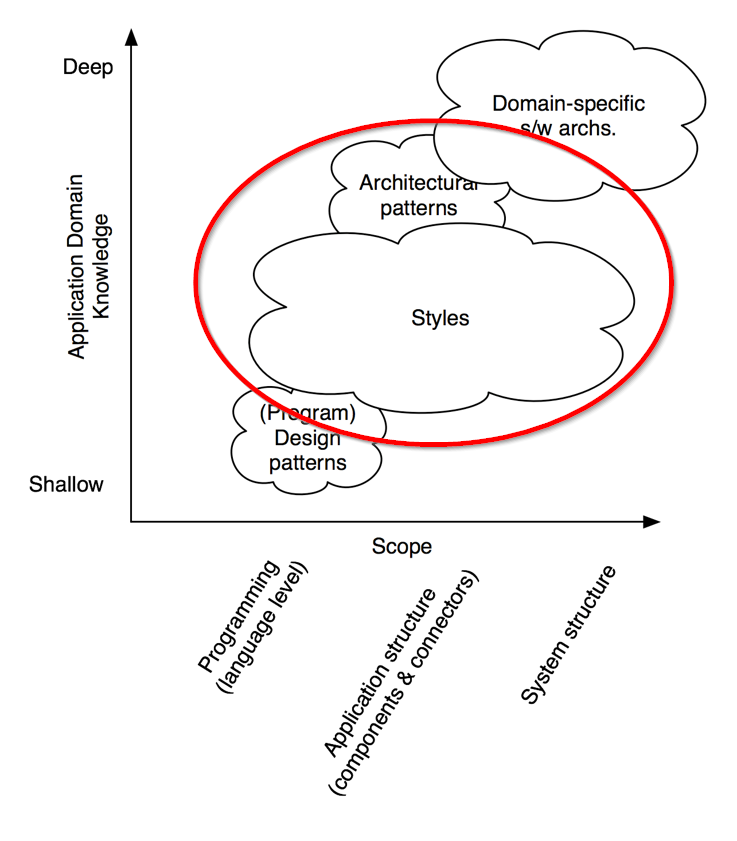
\includegraphics[width=0.52\textwidth]{architecturalStylesHighlighted.png}
    \attribution{N. Medvidovic}
\end{center}

Паттерны проектирования, которые мобсуждались в предыдущих лекциях --- самые <<тактические>> элементы архитектуры. Они никак не привязаны к предметной области и появляются на уровне реализации небольших подсистем или даже конкретных классов. Архитектурные стили, о которых в основном пойдёт речь сегодня, применимы уже не для всех проектов вообще, а в предпочтительных для каждого стиля предметных областях --- одни стили хорошо работают во встроенных системах, другие --- сетевых приложениях, третьи --- в информационных системах (отсюда <<применимы в выбранном контексте разработки>> из определения). И решения, диктуемые стилями, применяются не на уровне конкретных классов, а на уровне подсистем или даже целой системы.

Архитектурные шаблоны --- это более специализированная вещь, чем стили, и несколько более <<тактическая>> (хотя и не настолько, как паттерны). Архитектурные шаблоны диктуют типовые решения для типовых задач, например, организация системы в виде тройки Sense-Compute-Control в робототехнике, или Model-View-Controller в пользовательских интерфейсах. Model-View-Controller не претендует на то, чтобы диктовать архитектуру всего приложения, и тем отличается от архитектурных стилей --- обычно MVC лишь вершина айсберга, ответственная за общение с пользователем, а настоящая Архитектура начинается на уровне бизнес-логики, с которым работает Model.

Ещё выше по масштабности и глубже по погружению в предметную область находятся предметно-ориентированные архитектуры или Reference Architectures (например, Space AVionics Open Interface aRchitecture от ESA, Connected Vehicle Reference Implementation Architecture и т.д. и т.п.). В каждой предметной области они свои и, как правило, даже диктуются стандартами. Рассматривать их в этом курсе мы не будем в силу их чрезмерной специфичности.

\section{Архитектурные шаблоны}

Вот несколько примеров архитектурных шаблонов. Они тоже специфичны для предметных областей, но некоторые часто встречающиеся достойны рассмотрения.

\subsection{State-Logic-Display}

\noindent\begin{minipage}{\textwidth}
    \begin{minipage}[c][6cm][c]{\dimexpr0.7\textwidth-0.5\Colsep\relax}
        State-Logic-Display, также известный как <<трёхзвенная архитектура>>, часто рассматривается как архитектурный стиль, часто --- как архитектурный шаблон, так что вообще разделение на архитектурные шаблоны и архитектурные стили весьма условно. Многие приложения могут целиком быть реализованы по трёхзвенной схеме, причём ни в одном из этих звеньев не будет содержательной архитектурной сложности, тогда это что-то вроде стиля. Если трёхзвенка --- это только способ решения одной из задач, то это архитектурный шаблон. Вообще, трёхзвенка предполагает разделение приложения на часть, отвечающую за представление и взаимодействие с пользователем (и ничего больше), бизнес-логику и слой хранения данных.
    \end{minipage}\hfill
    \begin{minipage}[c][6cm][c]{\dimexpr0.3\textwidth-0.5\Colsep\relax}
        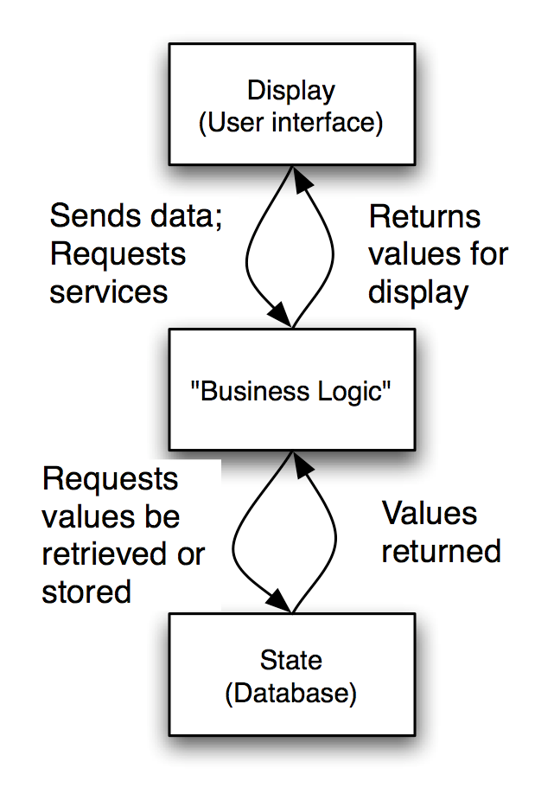
\includegraphics[width=0.9\textwidth]{threeTieredArchitecture.png}
    \end{minipage}%
\end{minipage}

Наличие чёткого разделения ответственности между слоями делает каждый из них управляемым, а функциональность --- переипользуемой. Например, пользовательский интерфейс легко поменять, сделав вместо десктопного приложения мобильное, не меняя бизнес-логики. В больших приложениях все три части могут быть физически размещены на разных машинах, причём пользовательских клиентов может быть много и они все работают со слоем бизнес-логики, который один. Или можно иметь несколько серверов с бизнес-логикой, лишь бы они смотрели на одну базу данных. Которая тоже может быть распределённой, так что это очень хорошо сказывается на масштабировании. 

Главные архитектурные ограничения --- клиент не знает ничего о БД и не может с ней напрямую взаимодействовать, бизнес-логика сама не пытается хранить информацию и не содержит ничего, что касается взаимодействия с польззователем, база данных не пытается делать ничего нетривиального с данными. 

Приложения, устроенные таким образом --- это подавляющее большинство веб-приложений и информационных систем (которые чаще всего сами веб-приложения), многопользовательские игры. В них клиент может быть очень продвинутым и очень сложным, но он не вправе заниматься реализацией игровой логики и не может хранить данные, кроме тех, что относятся к взаимодействию с пользователем (например, его логин).

\subsection{Model-View-Controller}

Model-View-Controller --- это архитектурный шаблон, который иногда классифицируют как паттерн проектирования: собственно, в книжке про паттерны Эриха Гамма со товарищи с него и начинается изложение. Так что даже разделение на паттерны и архитектурные шаблоны тоже весьма условно. Кажется, что это всё-таки что-то большее, чем паттерн, поскольку он не предписывает наличия конкретных классов, да и сам часто реализуется через некоторые паттерны (например, <<Наблюдатель>>, <<Команда>>).

Архитектурный шаблон устроен следующим образом:

\begin{center}
    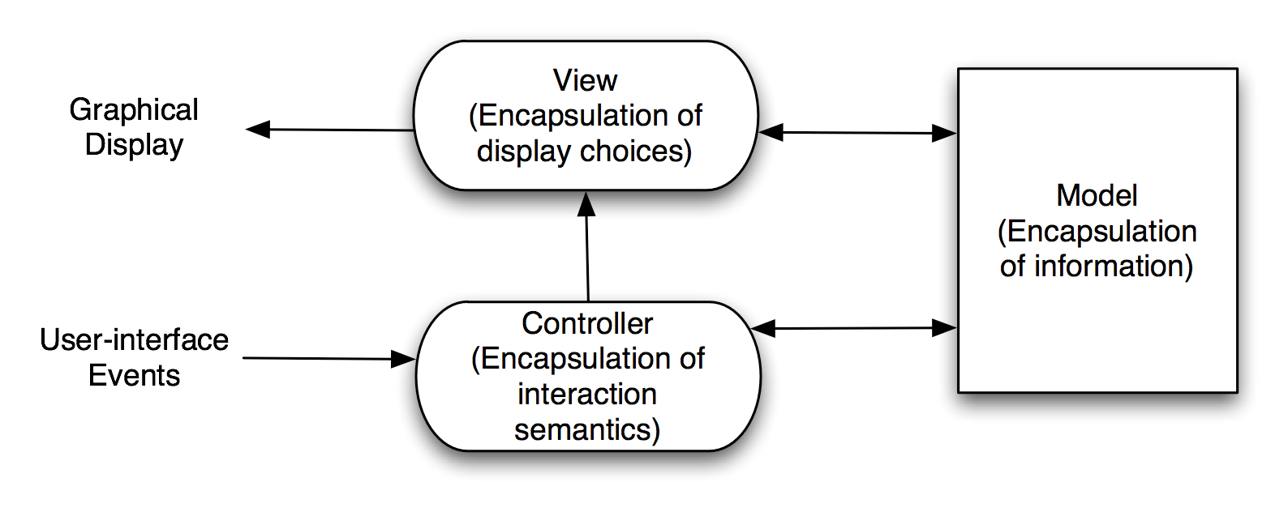
\includegraphics[width=0.75\textwidth]{mvc.png}
    \attribution{N. Medvidovic}
\end{center}

View отвечает за отображение данных пользователю и только за это. Пользовательский ввод поступает в Controller, ответственность которого --- обеспечить логику взаимодействия с пользователем и при необходимости управлять для этого View. Model --- компонент, хранящий в себе все данные и, как правило, включающий в себя также и бизнес-логику приложения. Контроллер обрабатывает пользовательский ввод, сообщает о требуемых действиях можели, модель их выполняет, меняет данные и рассылает нотификацию о том, что в ней что-то изменилось. Эту нотификацию получает представление, читает информацию из модели и обновляет себя.

Архитектурные ограничения: представление может только читать из модели, команды модели может отдавать только контроллер. Сигнал об обновлениях модель рассылает сама, что позволяет иметь несколько разных представлений, отображающих одну модель, которые будут синхронно обновляться. Контроллер --- единственное место системы, через которое проходят все команды пользователя.

Чем это хорошо --- так же, как в трёхзвенке, имеется чёткое разделение ответственности между компонентами и возможность выкинуть представление (или контроллер) и заменить на новое. Кроме того, контроллер --- это естественное место для реализации функцинальности Undo/Redo и обычно реализуется с помощью паттерна <<Команда>>. 

Model-View-Controller отличается от трёхзвенки тем, что не специфицирует, кому где хранить данные (поэтому применим в приложениях, которым данные особо хранить не надо), но требует наличия выделенного элемента, отвечающего за обработку пользовательского ввода (в трёхзвенке это делал Display, вместе с выводом информации).

Типичные приложения, построенные по такому принципу --- это большинство десктопных приложений с развитым пользовательским интерфейсом. Как правило, впрочем, Model-View-Controller является лишь малой частью их архитектуры, а вся логика и вся архитектурная сложность скрыта под Model.

\subsection{Sense-Compute-Control}

Sense-Compute-Control --- архитектурный шаблон, применяющийся прежде всего в робототехнике и схожих областях (например, <<умных домах>>). Он предполагает разделение работы системы на три фазы ---- снятие показания с датчиков, вычисление управляющего воздействия, посылка управляющего воздействия на актуаторы:

\begin{center}
    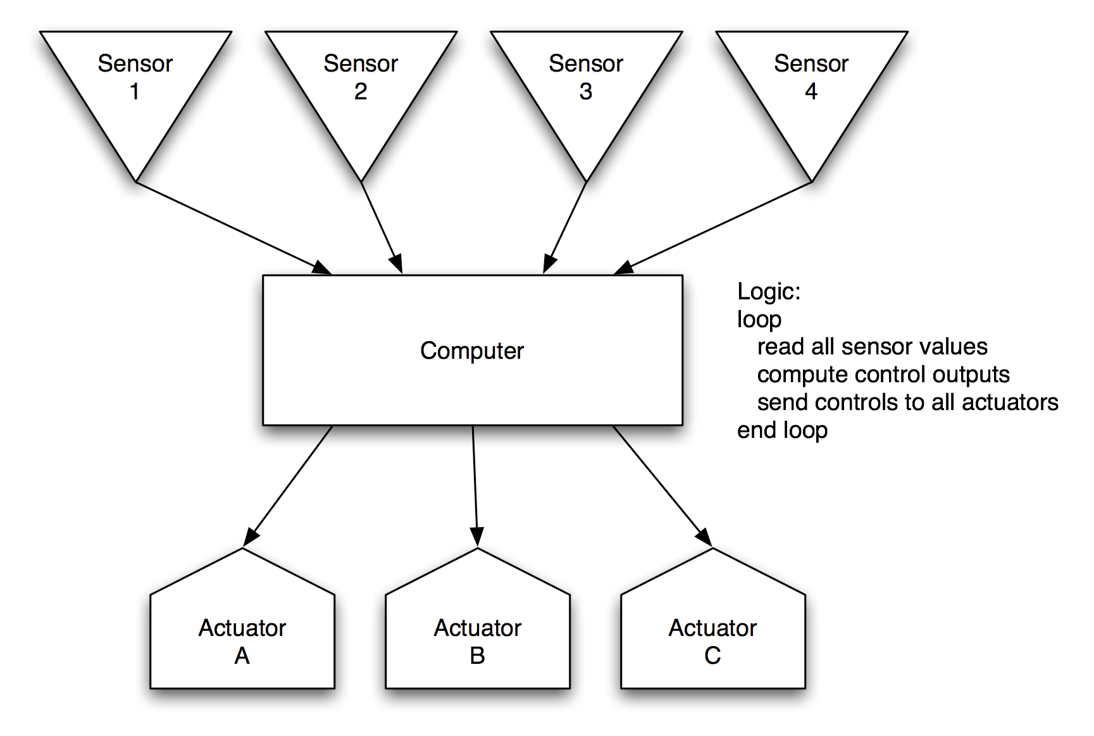
\includegraphics[width=0.65\textwidth]{senseComputeControl.png}
    \attribution{N. Medvidovic}
\end{center}

При этом вся система работает в бесконечном цикле, попеременно выполняя эти три фазы.

Очень простые системы (например, робот, едущий по датчику расстояния вдоль стенки) на самом деле больше ничего интересного не содержат, но в общем случае фаза Compute может включать в себя построение и обновление модели внешнего мира (например, целый большой и страшный SLAM\footnote{Simultaneous Localization And Mapping}), кучу сложной логики по определению поведения исходя из текущей модели мира и новых данных сенсоров.

Хорошо это тем, что чётко определяет архитектуру системы и для простых систем фактически решает все архитектурные вопросы. Для сложных систем это может быть только самый внешний каркас процесса работы, но поэтому это и не архитектурный стиль, а всего лишь шаблон.

\section{Архитектурные стили}

\noindent\begin{minipage}{\textwidth}
    \begin{minipage}[c][6cm][c]{\dimexpr0.5\textwidth-0.5\Colsep\relax}
        Архитектурные стили менее специализированы, чем архитектурные шаблоны. Так же, как и шаблоны, стили имеют имя и набор известных свойств, которые позволяют выбрать стиль, подходящий под решение задачи. Архитектурные стили в разработке ПО часто сравнивают с архитектурными стилями в архитектуре. Так же, как в архитектуре, стили могут быть совсем разными, при этом решать схожие задачи и, в конечном итоге, быть отражением вкусовых предпочтений архитектора.
    \end{minipage}\hfill
    \begin{minipage}[c][6cm][c]{\dimexpr0.5\textwidth-0.5\Colsep\relax}
        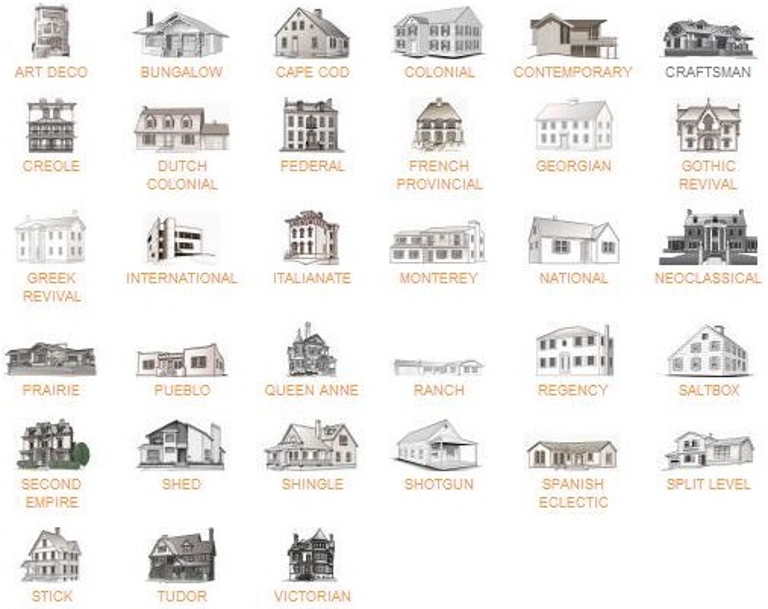
\includegraphics[width=0.9\textwidth]{buildingStyles.png}
        \attribution{N. Medvidovic}
    \end{minipage}%
\end{minipage}

Однако не все архитектурные стили хороши для всех ситуаций. Пример, который приводил N. Medvidovic в своей лекции --- в Калифорнии делают лёгкие каркасные дома из деревянного бруса, а в Сербии, откуда он родом --- большие дома из камня, передающиеся из поколения в поколение. Дело в том, что в Калифорнии высока сейсмическая активность, которая деревянным домам не страшна, а каменные бы и пары лет не простояли. В Сербии землетрясений не бывает, а камня в достатке.

\noindent\begin{minipage}{\textwidth}
    \begin{minipage}[c][6cm][c]{\dimexpr0.6\textwidth-0.5\Colsep\relax}
        При этом одна система вполне может включать в себя несколько разных архитектурных стилей (опять-таки, по аналогии со строительством, где есть, например, разные архитектурные стили крыши). Для каждой подсистемы стиль может быть свой. Например, система может быть организована в слоистом стиле, но слой бизнес-логики реализован в стиле Pipes and Filters, а слой пользовательского интерфейса --- в стиле <<ядро и плагины>>. Тем не менее, обычно прослеживается некий <<главный>> стиль --- высокоуровневая структура системы, которая и связывает компоненты, потенциально написанные очень по-разному.
    \end{minipage}\hfill
    \begin{minipage}[c][6cm][c]{\dimexpr0.4\textwidth-0.5\Colsep\relax}
        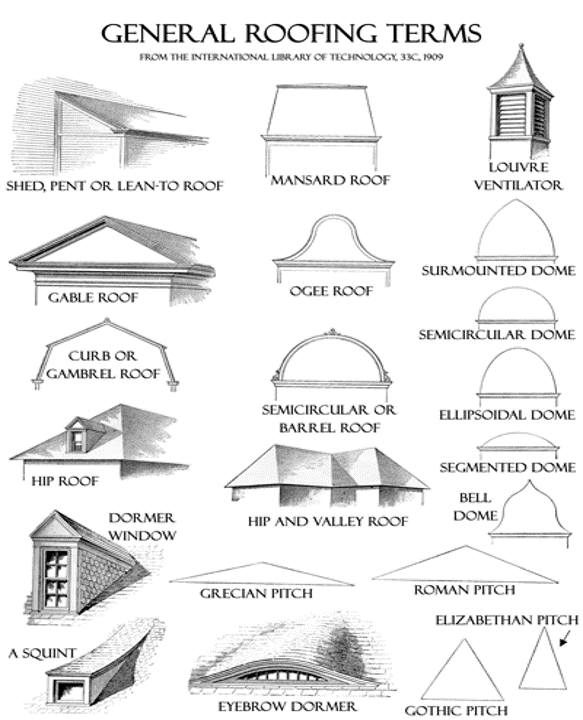
\includegraphics[width=0.9\textwidth]{roofStyles.png}
        \attribution{N. Medvidovic}
    \end{minipage}%
\end{minipage}

Архитектурные стили используются, чтобы получить следующие преимущества.

\begin{itemize}
    \item Переиспользование архитектуры. Создание архитектуры может быть сложной задачей, особенно когда у вас есть только требования и <<чистый лист>>. Выбор стиля сужает пространство решений и направляет архитектурную мысль. При этом для новых задач можно применять хорошо известные и изученные решения, обладающие известными достоинствами и недостатками применительно к вашей ситуации.
    \item Переиспользование кода. Часто у архитектурных стилей бывают неизменяемые части, которые можно один раз реализовать, а затем переиспользовать в каждой системе. Трёхзвенная архитектура, например, реализуется многими библиотеками для разработки веб-приложений, для событийно-ориентированных стилей есть хороший middleware (например, уже упоминавшийся ROS), дря распределённых стилей --- технологии наподобие gRPC или WCF, и т.д. Это существенно сокращает затраты на разработку.
    \item Упрощение общения и понимания системы. Как и в случае с паттернами, достаточно просто назвать стиль по имени и не надо объяснять, как что устроено --- опытные разработчики вас сразу поймут.
    \item Упрощение интеграции приложений, на тактическом уровне за счёт переиспользования стандартов и middleware, типичных для стиля, на стратегическом --- за счёт того, что понятно, куда и как встраиваться, не нарушив архитектурные ограничения каждого из приложений.
    \item Применение специфичных для стиля методов анализа. Поскольку стили накладывают ограничения на структуру систем, иногда эти ограничения достаточно жёсткие, чтобы про систему можно было что-то доказать или что-то посчитать. Хороший пример в этом плане --- стиль Pipes and Filters, к которому применимы алгоритмы анализа графов, которые можно использовать для анализа пропускной способности системы, её надёжности и т.п.
    \item Специфичные для стиля методы визуализации --- тот же Pipes and Filters удобно рисовать с помощью визуальных языков, ориентированных на данные, таких как Data Flow Diagram. Или становится возможным использование предметно-ориентированных языков --- например, на том же Pipes and Filters построено программирование в LabVIEW и Matlab/Simulink. Pipes and Filters тут не исключение, например, Microsoft Robotics Developer Studio имела по сути визуальный DSL для создания программ в распределённом веб-сервисном стиле.
\end{itemize}

Все стили фиксируют ограничения на возможные архитектуры, и какие именно эти ограничения --- и есть описание стиля. Стили определяются тремя основными соображениями: набор используемых в стиле элементов, набор правил, по которым эти элементы соединяются, и семантика, стоящая за элементами. Элементы могут быть компонентами, соединителями, элементами данных и т.п., например, некоторые стили описывают объекты и вызовы методов, некоторые --- сервера и каналы связи, некоторые --- фильтры и каналы данных. Правила соединения элементов --- это набор <<топологических>> ограничений на то, кто с кем может соединяться, и это, как правило, и есть самая суть стиля. Например, строгий слоистый стиль требует, чтобы элементы одного слоя могли общаться только друг с другом и с элементами слоя ниже. Семантика, стоящая за элементами, ограничивает их возможности, например, фильтрам можно запретить иметь собственное состояние, а каналам --- преобразовывать данные.

Дальнейшее рассмотрение будет вестись на одном примере (далеко не для всех стилей подходящем, но так даже веселее) --- игре <<посадка на луну>>, распространённой на игровых автоматах в 80-е.

\noindent\begin{minipage}{\textwidth}
    \begin{minipage}[c][6cm][c]{\dimexpr0.6\textwidth-0.5\Colsep\relax}
        Суть игры в том, что у вас есть спускаемый аппарат с двигателем, тягой которого можно управлять, ограниченный запас топлива и необходимость мягко (с вертикальной скоростью не болше заданной) посадить аппарат на поверхность планеты. При этом при старте игры задано количество топлива и начальная скорость аппарата --- естественно, так, чтобы топлива хватало как раз на оптимальную посадку, поэтому игра на самом деле может быть весьма сложной. 
    \end{minipage}\hfill
    \begin{minipage}[c][6cm][c]{\dimexpr0.4\textwidth-0.5\Colsep\relax}
        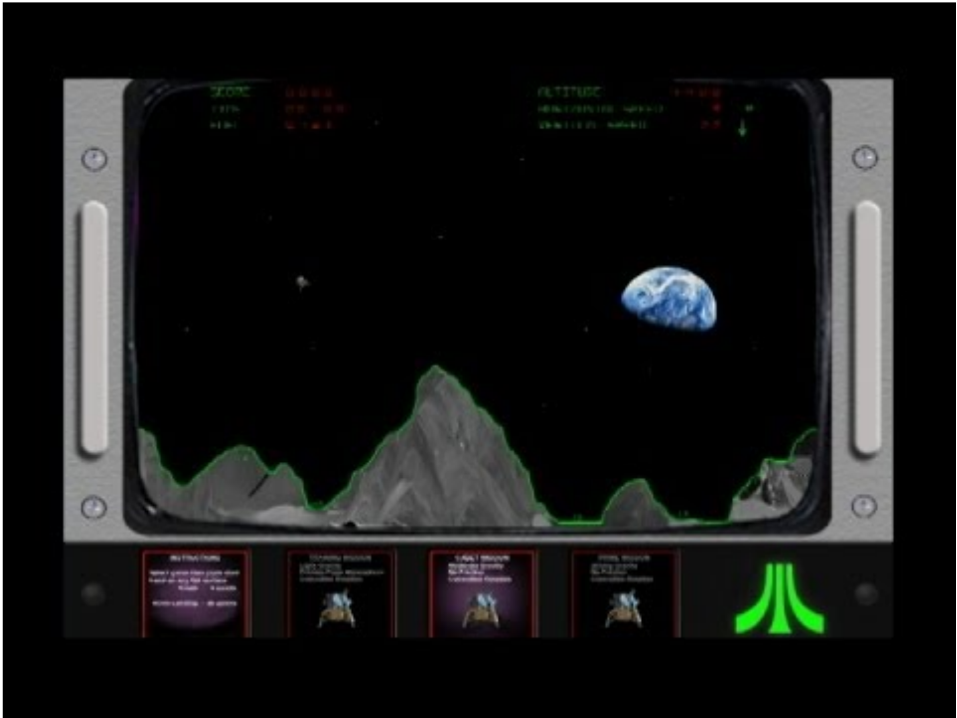
\includegraphics[width=0.9\textwidth]{lunarLander.png}
        \attribution{N. Medvidovic}
    \end{minipage}%
\end{minipage}

Продвинутые версии позволяли также управлять горизонтальным движением аппарата (например, поворотом маршевого двигателя), что делало игру ещё сложнее, потому что надо было выбрать горизонтальную поверхность для посадки.

Например, Lunar Lander в Sense-Compute-Control-стиле мог бы иметь такую архитектуру:

\begin{center}
    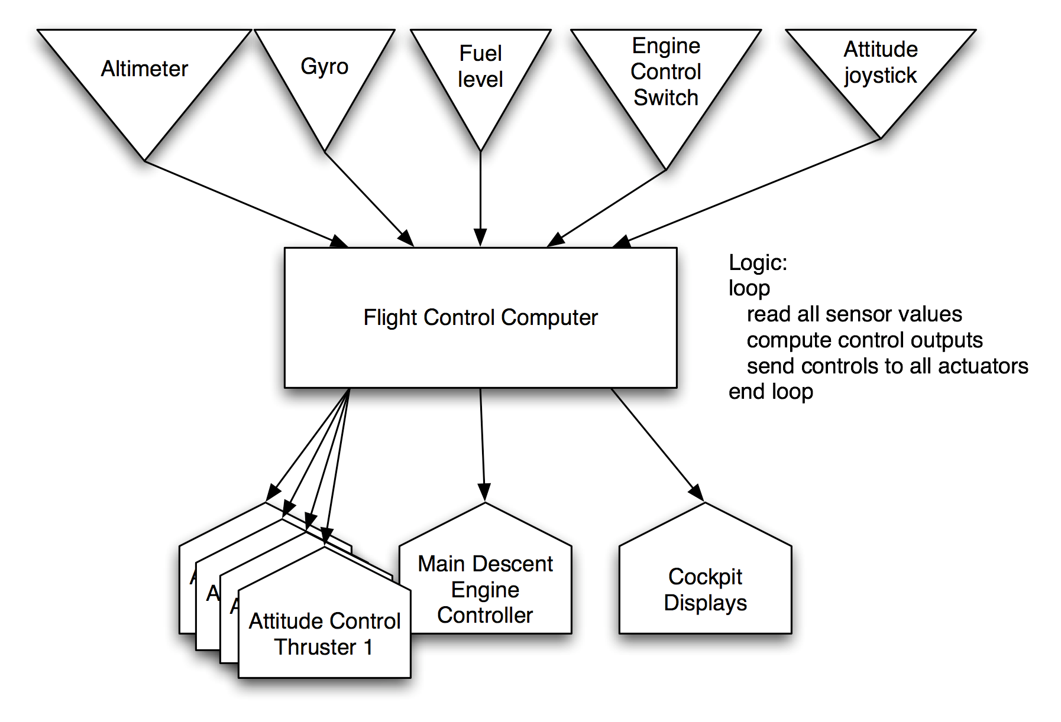
\includegraphics[width=0.8\textwidth]{senseComputeControlLunarLander.png}
    \attribution{N. Medvidovic}
\end{center}

Есть компоненты, отвечающие за симуляцию сенсоров аппарата, есть борткомпьютер, отвечающий за вычисление управляющего воздействия, есть актуаторы --- маневровые двигатели, маршевый двигатель, дисплеи приборов в кабине. Игра на игровых автоматах такую глубину симуляции, наверное, не обеспечивала, но если бы мы хотели сделать максимально реалистичную игру, её компонент, отвечающий за симуляцию самого аппарата, мог бы выглядеть как-то так.

Дальше речь пойдёт про следующие стили.

\begin{itemize}
    \item ``Традиционные'', связанные с языком: 
    \begin{itemize}
        \item главная программа/подпрограммы --- наследие структурных языков программирования, до сих пор вполне применяется при написании небольших утилит, драйверов и т.п.
        \item объектно-ориентированный --- точнее <<сырой>> объектно-ориентированный стиль, предполагающий докомпозицию программы на взаимодействующие объекты без дополнительных ограничений. Многие другие стили уточняют этот.
    \end{itemize}
    \item Уровневый стиль и его уточнения:
    \begin{itemize}
        \item виртуальные машины,
        \item уже знакомая нам трёхзвенная архитектура,
        \item клиент-сервер.
    \end{itemize}
    \item Стили, ориентированные на поток данных:
    \begin{itemize}
        \item пакетное исполнение,
        \item каналы и фильтры.
    \end{itemize}
    \item Peer-to-peer --- стиль разработки распределённых приложений. Сегодня про него упомянем, как дойдём до распределённых приложений, рассмотрим подробнее.
    \item Стили с общей памятью, более конкретно --- Blackboard.
    \item <<Интерпретатор>> и <<мобильный код>> --- стили, строящиеся вокруг исполнения стороннего кода в наиболее подходящем для этого месте.
    \item Стили с неявным вызовом:
    \begin{itemize}
        \item <<чистый>> событийно-ориентированный стиль,
        \item событийно-ориентированный стиль с шиной событий,
        \item <<Издатель-подписчик>>.
    \end{itemize}
    \item <<Производные>> стили, являющиеся уточнением и комбинацией существующих:
    \begin{itemize}
        \item распределённый объектно-ориентированный стиль (идея за технологиями типа CORBA),
        \item REST,
        \item Components and Connectors (C2).
    \end{itemize}
\end{itemize}

\subsection{Главная программа/подпрограммы}

Главная программа/подпрограммы --- стиль, опирающийся на функциональную декомпозицию. Задача разбивается на подзадачи, каждая из которых решается отдельной функцией, которая в свою очередь может вызывать другие функции и т.д., пока задачи не станут достаточно простыми. Стиль хорош простотой и предсказуемостью поведения системы, скоростью работы. Плох тем, что для любой нетривиальной задачи функций (и даже уровней декомпозиции) получится существенно больше, чем можно удержать в голове, и между ними потребуется передавать данные (опять-таки, в очень больших количествах), которым очень сложно обеспечить инкапсуляцию. В общем, такой подход реально хорошо подходит для небольших систем, но если получается больше нескольких тысяч строк кода, всё становится плохо управляемым.

Формально компонентами в таком стиле являются функции, соединителями --- вызовы, с передачей параметров, ограничениями --- обычно граф вызовов должен образовывать ориентированный ациклический граф, но при необходимости колбэков и взаимной рекурсии это ограничение может нарушаться (что несколько усложняет анализ программы).

Lunar Lander в таком стиле мог бы быть спроектирован так:

\begin{center}
    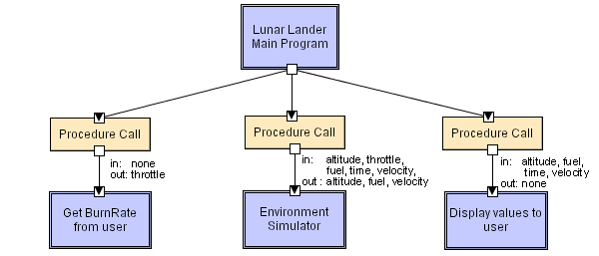
\includegraphics[width=0.8\textwidth]{mainProgramAndSubroutinesLL.png}
    \attribution{N. Medvidovic}
\end{center}

\subsection{Объектно-ориентированный стиль}

<<Сырой>> объектно-ориентированный стиль --- когда программа представляется в виде набора взаимодействующих объектов в обычном объектно-ориентированном стиле. Компонентами в этом стиле выступают объекты, соединителями --- вызовы методов, ограничения --- объекты должны полностью контролировать своё внутреннее состояние и менять его можно только через вызовы методов, при этом реализация этих методов должна быть полностью скрыта от других объектов. В общем, обычные требования ООП.

Я бы вообще не называл объектно-ориентированный стиль архитектурным стилем, поскольку он почти никаких ограничений не накладывает, но тем не менее, можно говорить об его достоинствах и недостатках. Достоинства --- прежде всего, близость к предметной области и <<обычному>> человеческому мышлению. Сущности предметной области и так имеют своё состояние и поведение, это более-менее прямолинейно ложится в код. Кроме того, с точки зрения техники программирования каждый объект независим, так что его можно разрабатывать отдельно, и главное, думать о нём отдельно: рассматривать систему как набор взаимодействующих агентов, которые вместе решают задачу, но каждый из них более-менее обособлен, его можно отдельно разрабатывать и отдельно тестировать. Ещё одно важное тактическое соображение --- реализацию объектов можно смело менять, пока выполняются их инварианты, во внешнем мире это гарантированно ничего не сломает.

Есть и недостатки. Главный --- это, пожалуй, отсутствие строгих топологических ограничений на связи между объектами, что приводит к тенденции <<чистых>> объектно-ориентированных программ превращаться в месиво из объектов, где каждый вынужден знать о каждом. Поэтому при программировании в чистом объектно-ориентированном стиле обязательно создание высокоуровневой структуры системы или применение дополнительных стилей, которые её диктуют, например, слоистого.

Второй недостаток (по сравнению с функциональным программированием, по крайней мере, и даже со структурным) --- сколоность к побочным эффектам. Методы обычно меняют состояние объекта, так что разная последовательность вызовов одних и тех же методов с одними и теми же параметрами приводит к разным результатам. Это существенно усложняет анализ.

Lunar Lander в таком стиле мог бы быть спроектирован так:

\begin{center}
    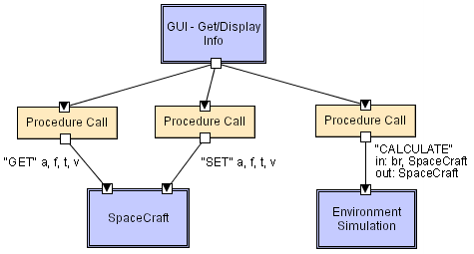
\includegraphics[width=0.7\textwidth]{objectOrientedLL.png}
    \attribution{N. Medvidovic}
\end{center}

Или, в более формальной нотации диаграмм классов UML:

\begin{center}
    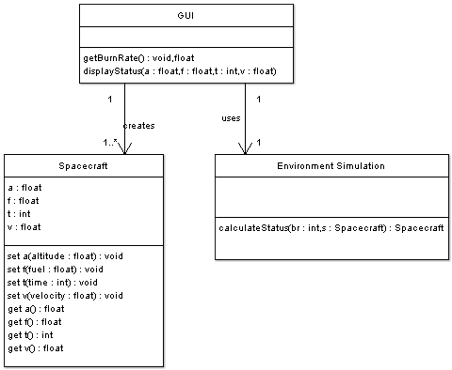
\includegraphics[width=0.7\textwidth]{objectOrientedLLUML.png}
    \attribution{N. Medvidovic}
\end{center}

\subsection{Слоистый стиль}

\noindent\begin{minipage}{\textwidth}
    \begin{minipage}[c][10cm][c]{\dimexpr0.8\textwidth-0.5\Colsep\relax}
        Перейдём к рассмотрению <<настоящих>> архитектурных стилей. Первый такой стиль, а точнее даже группа стилей --- это слоистый стиль и его возможные вариации. Суть этого стиля в том, что мы разделяем систему на слои, где каждый слой может пользоваться слоями ниже и предоставляет интерфейс для слоёв выше, при этом сам ничего о них не зная. Его можно понимать как <<многоуровневый клиент-сервер>> в том смысле, что каждый слой выступает клиентом слоёв ниже и сервером для слоёв выше. Компонентами в таком стиле выступают сами слои, они могут быть сколь угодно сложно устроены внутри, но это их детали реализации. Соединителями --- протоколы общения слоёв (или просто программные интерфейсы). Примеры слоистых архитектуры мы уже видели: трёхзвенная архитектура, также по такому принципу устроены сетевые стеки (модели OSI и TCP/IP состоят из слоёв протоколов), операционные системы, многие бизнес-приложения. Lunar Lander в таком стиле мог бы выглядеть так, как на рисунке справа.

        \vspace{3mm}

        Преимущества слоистого стиля --- это в первую очередь постепенное повышение уровня абстракции от низких уровней к высоким. В строгом варианте, когда слой может общаться только со слоем непосредственно ниже, это позволяет вообще не думать о  реализации всей системы, а просто программировать в терминах предоставляемой слоем абстракции (так, например, реализуются сетевые приложения, вы просто пользуетесь сокетами или высокоуровневыми протоколами и не интересуетесь тем, что происходит на уровнях глубже).
    \end{minipage}\hfill
    \begin{minipage}[c][10cm][c]{\dimexpr0.2\textwidth-0.5\Colsep\relax}
        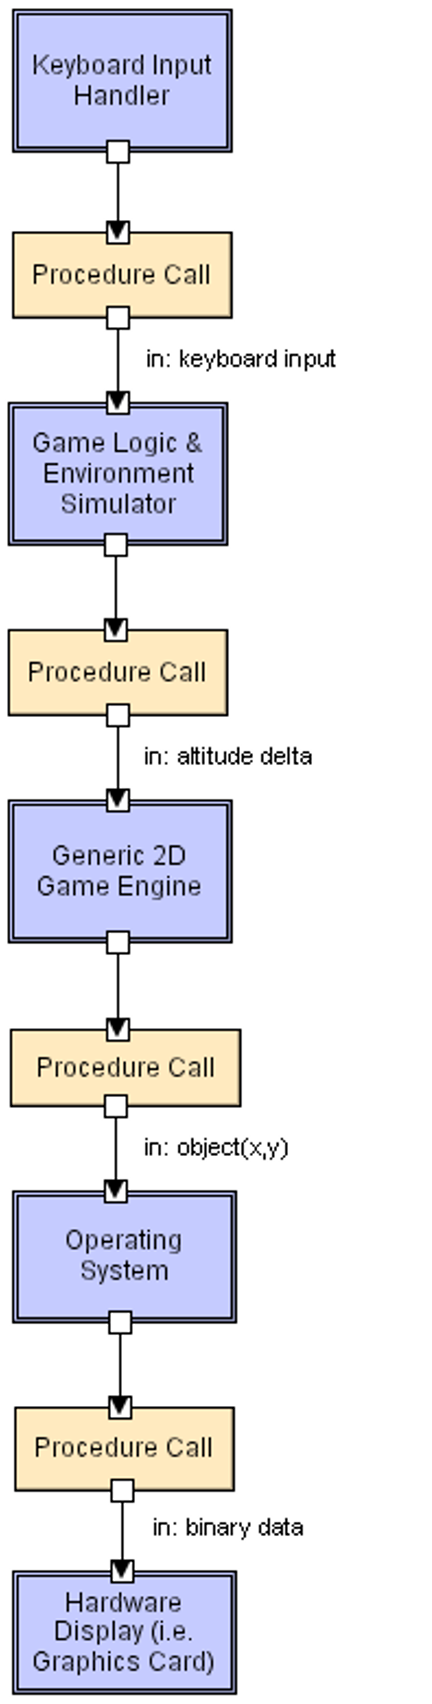
\includegraphics[width=0.9\textwidth]{layeredLL.png}
        \attribution{N. Medvidovic}
    \end{minipage}%
\end{minipage}

Ещё слоистость существенно облегчает сопровождение системы. Поскольку каждый уровень влияет только на уровни выше, влияние каждого изменения легко оценить и отследить. При этом можно использовать разные реализации каждого уровня, лишь бы они удовлетворяли общему интерфейсу --- примером этого снова являются сетевые приложения, мы можем использовать на физическом уровне Ethernet или WiFi, совершенно ничего не меняя уровнями выше. То же касается драйверов операционной системы --- мы можем использовать низкоуровневую графическую библиотеку типа OpenGL для вывода графики, не зная, что за видеокарта у пользователя, был бы драйвер. Да и саму библиотеку можно поменять (на DirectX или Vulcan), если у нас есть высокоуровневый графический движок, оборачивающий низкоуровневые интерфейсы (например, Unity или UnrealEngine).

Однако есть и проблемы. Во-первых, уровневый стиль оказывается не всегда применим --- взаимодействие между элементами системы может быть таким, что не позволяет себя упорядочить по уровням. Пример тому был на первой лекции, с ПО к осциллографу, там уровневый стиль формально можно было навести, но данные шли <<вверх>> по уровням, а команды от пользователя --- <<вниз>>, так что все части ситемы всё равно были вынуждены знать про все остальные. Такие ситуации в реальной жизни встречаются, и тогда пыытаться натянуть уровневый стиль на систему не стоит. 

Во-вторых, проблемой может стать производительность системы. Сложные уровневые архитектуры имеют тенденцию обрастать функциями, которые просто прокидывают запрос на уровень ниже, что ведёт к ненужному оверхеду на вызовы. Если производительность критична, уровневый стиль может всё-таки хорошо подойти, но может и нет (особенно, если перестараться с количеством уровней). 

Тем не менее, уровневость --- это хорошо, поэтому иногда стоит даже проделать дополнительную работу, чтобы разделить систему на уровни. Уровневая архитектура считается довольно стандартной и, например, профстандарт профессии <<архитектор>> даже подразумевает её как архитектуру по умолчанию.

\subsection{Клиент-сервер}

<<Клиент-сервер>> --- это в каком-то смысле вырожденный случай уровневой архитектуры, когда уровня всего два. Собственно, клиенты и сервер --- это компоненты такого архитектурного стиля, сетевые протоколы (обычно) --- соединители. Ограничения --- клиенты не могут общаться друг с другом и могут общаться только с сервером, сервер ничего не знает о клиентах до того момента, как они не начнут с ним взаимодействовать, даже их количество. 

Серверов, кстати, может быть много, это позитивно сказывается на масштабируемости системы, но привноссит дополнительные трудности синхронизации состояния серверов, о которых будет чуть подробнее позже, в части курса, относящейся к распределённым приложениям.

Стиль типичен для несложных веб-приложений, где клиентом обычно выступает браузерная часть приложения, мобильных сетевых приложений или, что может быть несколько неожиданно, операционных систем. Графическая подсистема Linux, например, реализована по клиент-серверной архитектуре, есть оконный сервер и приложения, которые шлют ему запросы на отрисовку графических примитивов.

С помощью такого стиля можно сделать мультиплеерный Lunar Lander:

\begin{center}
    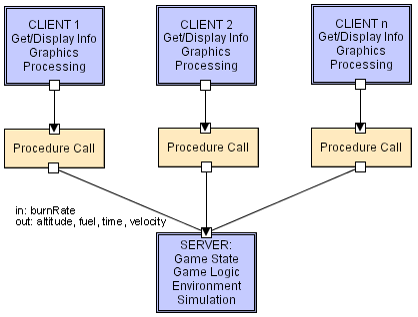
\includegraphics[width=0.7\textwidth]{clientServerLL.png}
    \attribution{N. Medvidovic}
\end{center}

\subsection{Пакетная обработка}

Пакетная обработка --- <<прадедушка архитектурных стилей>>, применявшийся ещё на заре массовой информатизации в финансовых системах глубокой древности:

\begin{center}
    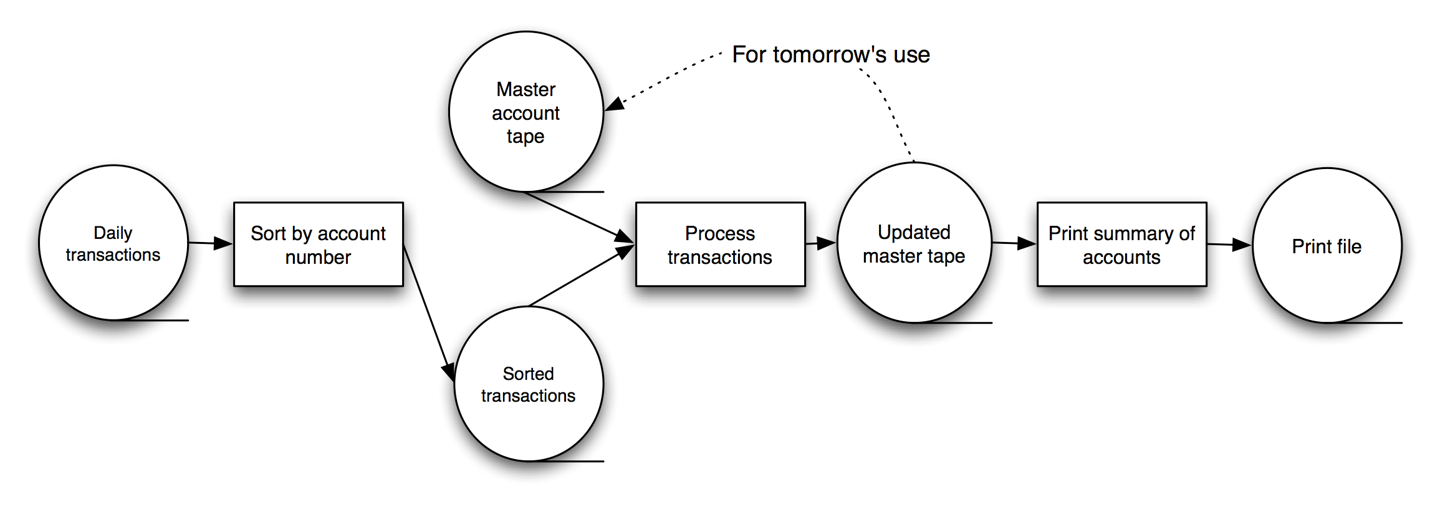
\includegraphics[width=0.9\textwidth]{batch.png}
    \attribution{N. Medvidovic}
\end{center}

Данные в те времена хранились на магнитных лентах (а это медленные устройства с последовательным доступом, перемотать ленту было целым делом). Данные о транзакциях за день подавались на вход программе сортировки, которая сортировала их по номерам аккаунтов, после чего выгружались на ленту с отсортированными транзакциями. Затем они и лента с данными об аккаунтах подавались на вход программе, которая проводит транзакции и сливает их в обновлённую ленту с аккаунтами (как в сортировке слиянием, для этого и надо было сначала транзакции отсортировать). Затем то, что получилось, подавалось на вход программе-печаталке, которая выдавала статистику по аккаунтам.

Итого, система в стиле <<пакетная обработка>> строится как набор отдельных программ, которые выполняются последовательно, обмениваясь данными средствами операционной системы. Это давно уже не ленты, а файлы, либо pipes или named pipes\footnote{Абстракция чего-то среднего между файлом и очередью сообщений, в неё можно писать одним процессом и вычитывать данные другим. Реально данные на диск не сохраняются, поэтому пайпы гораздо быстрее файлов как средство общения между процессами. Кстати, пайпы (даже именованные) поддерживаются и Windows, просто в Linux ими пользоваться удобнее}. При такой схеме между процессами требуется передавать в явном виде всё, что необходимо им для работы --- сами данные, конфигурацию, управляющие команды.

Стиль хоть и древний, но очень популярен до сих пор. По сути, Linux way с большим количеством маленьких утилит, из которых с помощью пайпов выстраиваются конвейеры --- это и есть пакетная обработка. Так что этот стиль применяется практически во всех скриптах под Linux и без него трудно представить работу системных администраторов, DevOps и т.д.

Важное преимущество этого стиля --- независимость отдельных программ. Они могут быть написаны на каком угодно языке и какой угодно технологии, лишь бы умели читать из входного потока. Можно их вообще не писать, а переиспользовать уже готовые в любой части конвейера. Этакая микросервисная архитектура внутри одной машины.

Важный недостаток этого стиля --- неторопливость работы. Каждая программа --- отдельный процесс, даже просто их запуск трудоёмок по времени и памяти, да и коммуникации между процессами, хоть и не так тяжелы, как коммуникации по сети, всё-таки гораздо медленнее общения потоков внутри процесса.

Lunar Lander в таком стиле мог бы выглядеть вот таким образом:

\begin{center}
    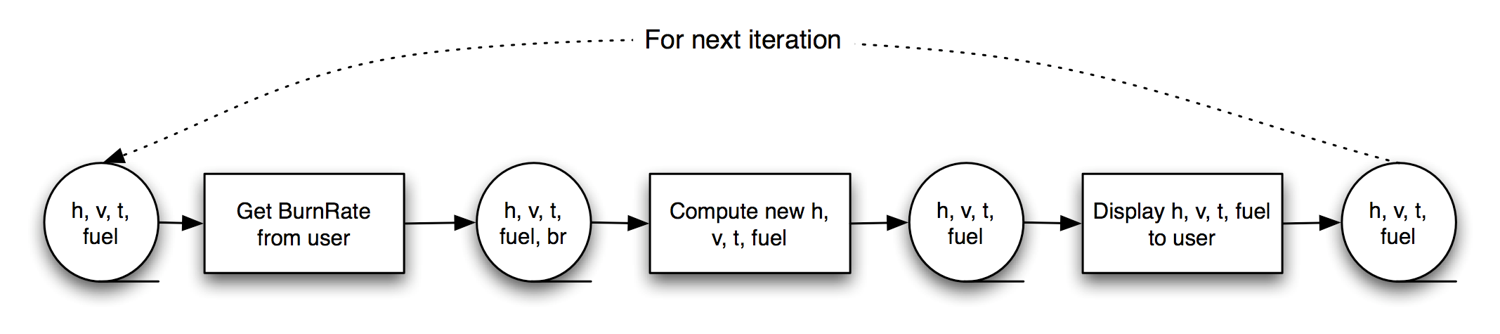
\includegraphics[width=0.9\textwidth]{batchLL.png}
    \attribution{N. Medvidovic}
\end{center}

Не уверен, что такая архитектура подошла бы для интерактивного приложения, но, ээ, как Play By Email бы, наверное, было неплохо. Некоторые пошаговые стратегии прошлого очень хорошо поддерживали Play By Email, хотя и вряд ли использовали пакетный стиль как архитектуру.

\subsection{Каналы и фильтры}

Каналы и фильтры (или <<pipes and filters>>) --- стиль, в котором программа представляется в виде набора фильтров, которые как-то преобразуют данные, идущие по каналам. При этом фильтры независимы друг от друга, то есть не имеют разделяемого состояния и ничего не знают про фильтры до и после них. Всё, что они видят --- это данные в своих входных каналах. Собственно, фильтры являются единственным типом элементов в такой архитектуре, а каналы --- единственным типом соединителей.

<<Каналы и фильтры>> похожи на <<пакетную обработку>>, но не требуют, чтобы каждый фильтр был отдельной программой, что помогает победить проблемы с производительностью в пакетной обработке. Кроме того, каналы и фильтры имеют тенденцию образовывать сложные сети, в отличие от пакетной обработки, где всё в основном линейно.

Бывают варианты каналов и фильтров:

\begin{itemize}
    \item конвейеры --- где фильтры связаны просто в линейную цепочку, очень топологически простой стиль, подходящий для несложной логики обработки (хотя сами фильтры могут быть сколь угодно сложны);
    \item ограниченные каналы --- где канал представляет собой очередь с ограниченным количеством элементов, блокирующую фильтр-источник, если очередь переполнена. На самом деле, лучше ограниченность каналов иметь в виду всегда, потому что фильтры, обрабатывающие данные с разной скоростью, могут привести к <<пробкам>> из данных на разных этапах обработки.
    \item Типизированные каналы --- где каналы знают тип передаваемых данных, и фильтры могут подключаться только к каналам правильного типа. Именно такой стиль в итоге был выбран в первой лекции этого курса в примере про осциллограф.
\end{itemize}

Преимущества этого стиля таковы.

\begin{itemize}
    \item Поведение системы --- это просто последовательное применение поведений компонентов. Так что о нём легко рассуждать, его легко понять, такие системы легко поддерживать.
    \item Легко добавлять, заменять и переиспользовать фильтры. Если не принимать в расчёт типизированные каналы, то вообще любые два фильтра можно использовать вместе. Если принимать, то любые два фильтра, у которых подходящие типы <<портов>>, можно использовать. Специально продумывать интеграцию компонентов не нужно, она получается сама собой.
    \item Широкие возможности для анализа. Поскольку есть чёткие ограничения на потоки данных, систему можно рассматривать просто как граф из фильтров с рёбрами-каналами, что делает применимыми все алгоритмы анализа графов. Можно считать пропускную способность системы, задержки (среднюю и максимальную), искать взаимные блокировки в сложных сетях.
    \item Широкие возможности для параллелизма. Каждый фильтр может работать одновременно со всеми остальными, либо в отдельном потоке, либо в отдельном процессе на другой машине (что, кстати, делает фильтры естественными кандидатами в микросервисы).
\end{itemize}

Недостатки тоже есть:

\begin{itemize}
    \item Последовательное исполнение --- что странно противоречит достоинству про параллелизм. Но пока первые фильтры из сети не сделают своё дело, следующие за ними к работе приступить не могут. Это не важно, когда данных много и вся сеть занята их обработкой, но если данные поступают лишь иногда, они должны последовательно пройти через все фильтры, при этом большая часть фильтров будет простаивать.
    \item Проблемы с интерактивными приложениями, поскольку данные идут по  фильтрам в одном направлении и непонятно, как ими управлять. Можно придумать <<обратные>> каналы управления, как это было в примере из первой лекции, но об этом надо специально думать и это несколько портит стройную картину этого стиля.
    \item Пропускная способность всей системы определяется самым ``узким'' элементом. Опять-таки, это можно обойти, масштабировав медленный фильтр, но это может быть технически непросто и об этом надо вовремя подумать.
\end{itemize}

Lunar Lander в этом стиле мог бы быть спроектирован вот так:

\begin{center}
    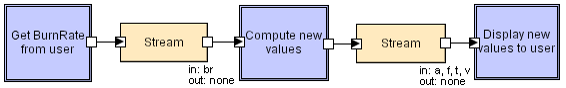
\includegraphics[width=0.7\textwidth]{pipesAndFiltersLL.png}
    \attribution{N. Medvidovic}
\end{center}

\subsection{Blackboard}

Blackboard --- это архитектурный стиль с общей памятью. Есть центральное хранилище данных, тот самый <<Blackboard>>, есть компоненты, которые знают только про Blackboard, не имеют своего состояния и, собственно, выполняют полезную работу. Процесс работы системы устроен так, что каждый компонент смотрит на Blackboard, (возможно) находит там данные, которые может преобразовать, преобразовывает их и записывает обратно на Blackboard, в надежде, что какой-то другой компонент сможет преобразовать их дальше. Это чем-то похоже на группу экспертов, которые решают задачу, сидя в одной комнате с доской --- каждый эксперт шарит только в своей предметной области, поэтому выходит к доске и пишет на ней что-то, что соответствует его экспертизе и, возможно, поможет другим экспертам решить задачу. 

Весь процесс вычислений управляется только через Blackboard, поэтому если мы хотим, чтобы некоторые действия выполнялись последовательно, нам надо хранить на Blackboard какой-то токен исполнения и обновлять его при выполнении действий.

Такой подход хорош тем, что компоненты могут быть полностью независимы и работать параллельно (и разрабатываться независимо, кстати), система легко масштабируется и расширяется добавлением новых компонентов, и главное, что вам не надо даже понимать алгоритм решения задачи --- вы просто бросаете в систему компоненты пока задача не решится. Это же и главный недостаток этого стиля --- задача легко может и не решиться. Поэтому такой стиль применяется прежде всего в системах искусственного интеллекта, где задача и так вполне может быть нерешаемой. Ещё, кстати, Blackboard, как правило, является узким местом системы, поскольку ему надо синхронизировать доступ независимы компонентов к себе.

Кстати, родственен Blackboard стиль, основанный на правилах переписывания --- например, машины Маркова и язык Рефал, графовые грамматики и подобные штуки. Там тоже есть центральная структура данных и набор правил, которые её независимо и постепенно изменяют. Такой подход вполне распространён и в <<обычной>> программной инженерии.

Lunar Lander в стиле Blackboard мог бы быть спроектирован вот так:

\begin{center}
    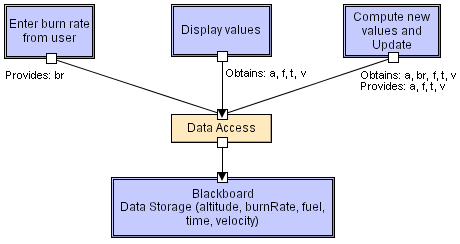
\includegraphics[width=0.7\textwidth]{blackboardLL.png}
    \attribution{N. Medvidovic}
\end{center}

\subsection{Стили с неявным вызовом}

Стили с неявным вызовом --- общее название разных вариантов событийно-ориентированных стилей или вообще стилей, где хотя бы иногда используются оповещения весто явных вызовов методов. Во всех таких стилях есть <<слушатели>>, которые могут подписываться на события, и при наступлении события система сама вызывает всех зарегистрированных слушателей.

В таких архитектурах компоненты имеют два вида интерфейсов --- обычный набор методов, и события, на которые можно подписываться. В качестве соединителей используются либо прямые вызовы методов, либо неявные вызовы слушателей по наступлению события (почему стили и называются стилями с неявным вызовом).

Инварианты всех таких стилей:

\begin{itemize}
    \item те, кто производит события, не знают, кто и как на них отреагирует --- они, как правило, технически имеют список подписавшихся, но обычно не вправе даже узнать их количество, не говоря уж о том, чтобы что-то делать с подписавшимися напрямую;
    \item не делается никаких предположений о том, как событие будет обработано и будет ли вообще --- источник просто нотифицирует систему о наступлении события, а уж подписан на него кто-нибудь или нет, в каком порядке кто подписан и т.д. --- не его дело.
\end{itemize}

Преимущества всех таких стилей --- это переиспользуемость компонентов и лёгкость конфигурирования системы. Высокая переиспользуемость достигается за счёт очень низкой связности между компонентами, ведь источник событий вправе вообще ничего не знать о тех, кто им пользуется. Лёгкость конфигурирования, как во время компиляции, так и во время выполнения, достигается за счёт того, что подписки на события можно легко менять, меняя при этом всю функциональность системы.

Недостатков, тем не менее, тоже довольно много.

\begin{itemize}
    \item Зачастую неинтуитивная структура системы. Без применения дополнительных архитектурных ограничений подписки на события превращаются в хаотичный клубок, в котором хаотично распространяются нотификации. Поэтому мы и рассмотрим конкретные стили, накладывающие дополнительные ограничения.
    \item Компоненты не управляют последовательностью вычислений. Работа системы состоит в генерации событий и реакций на события, и делать что-то в правильном порядке в сколько-нибудь сложной системе может оказаться проблематичным.
    \item Непонятно, кто отреагирует на запрос и в каком порядке придут ответы. Компонент, генерирующий события, не вправе предполагать, что на событие кто-то отреагирует, поэтому если это событие, например, <<мне нужны данные для дальнейшей работы>>, мы не вправе рассчитыввать на ответ. А если надо запросить несколько разных источнков, то неизвестно, кто и когда ответит. Поэтому такие системы принципиально асинхронны.
    \item Тяжело отлаживаться. Вы не можете просто сделать step into при вызове метода, вы должны мучительно ковыряться в списке подписчиков. Некоторые среды, типа C\#/Visual Studio, хорошо поддерживают отладку событий, но даже там, когда управление прыгает по всему коду, отлаживаться тяжело. К тому же, событийные системы принципиально асинхронны, что создаёт дополнительную боль.
    \item Ситуации, очень похожие на гонки, даже если у вас всего один поток. Классическая гонка --- это когда результат работы программы зависит от случайного порядка переключения потоков планировщиком. Гонка в событийных системах --- это когда результат работы программы зависит от случайного порядка вызова обработчиков при нотификации. Обычно событийные системы хоть и не позволяют закладывваться на определённый порядок вызова обработчиков, всё же вызывают их в порядке подписывания, что делает процесс хоть сколько-нибудь детерминированным. Но, во-первых, это не всегда возможно (например, в распределённых системах --- кто первый получил событие, тот его и обработал), во-вторых, порядок подписывания тоже такой себе ориентир --- на событие могут подписываться разные компоненты в разных частях кода, и помнить, кто когда должен подписаться, может оказаться слишком хлопотно. В таких местах особо часто появляется и особо опасен антипаттерн <<Sequential coupling>>.
\end{itemize}

\subsubsection{Издатель-подписчик}

<<Издатель-подписчик>> --- самый простой стиль из стилей с неявным вызовом, и вместе с тем весьма популярный и эффективный. Есть издатели, они публикуют сообщения (синхронно или асинхронно, то есть дожидаясь их обрабобтки либо нет). Есть подписчики, которые подписываются на издателей и получают от них события. Есть маршрутизаторы, задачча которых --- быть посредниками между издателями и подписчиками, фильтровать и маршрутизировать сообщения. При этом в самых простых конфигурациях без маршрутизаторов прекрасно обходятся, но они могут быть полезны: например, маршрутизатор может по очереди отправлять сообщения то одному подписчику, то другому, реализуя тем самым балансировку нагрузки.

Компонентами в таком архитектурном стиле являются издатели, подписчики и маршрутизаторы, соединителями --- сетевые протоколы или \textit{очереди сообщений}, либо, если дело происходит на одной машине, механизмы наподобие паттерна <<Наблюдатель>>. В качестве данных в этом стиле выступают подписки, нотификации о произошедших событиях, публикуемая издателями информация. Ограничения --- издатели ничего не знают о подписчиках, подписчики, как правило, ничего не знают друг о друге, только об издателях.

Преимущества этого стиля, как и обычно для событийно-ориентированных схем --- очень низкая связность между компонентами, но при этом высокая эффективность распространения информации, отчасти за счёт свойственной этому стилю простоты топологии, отчасти за счёт наличия маршрутизаторов.

Lunar Lander в этом стиле мог бы быть спроектирован вот так:

\begin{center}
    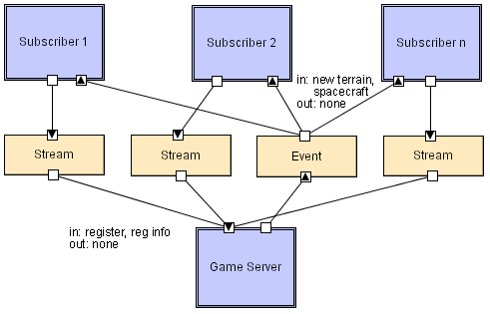
\includegraphics[width=0.7\textwidth]{pubSubLL.png}
    \attribution{N. Medvidovic}
\end{center}

\subsubsection{Событийно-ориентированный стиль с шиной}

Событийно-ориентированный стиль с шиной предполагает наличие шин событий, через которые могут общаться компоненты. При этом всё остальное как в чистых событийно-ориентированных стилях, есть компоненты, которые могут генерировать какие-то события и подписываться на чужие, но разница в том, что компоненты принципиально не могут взаимодействовать друг с другом напрямую, а общаются только через шину. Соответственно, подписаться можно только на события в шине, и посылать события можно только шине. При этом возможны два варианта взаимодействия --- <<push>>, когда шина сама активно уведомляет своих подписчиков, и <<pull>>, когда компоненты время от времени опрашивают шину на предмет наличия в ней новых событий. Шина в системе вполне может быть одна, но часто это несколько именованных шин с разными типами данных.

Преимущества такого подхода --- это ещё большая независимость компонентов, лёгкость машстабирования и добавления новой функциональности. Если кто-то не успевает обрабатывать запросы --- не проблема, подключим к шине ещё одну копию. Если нам надо новую функциональность, мы просто пишем компонент, подключаем его к шине и ничего больше в системе обычно менять не надо. Особенно эффективен такой стиль для распределённых приложений, где каждый компонент может быть отдельным сервисом. 

Пример дальнейшего уточнения такого стиля --- архитектурный паттерн интеграции <<Enterprise Service Bus>>, умная шина, позволяющая преобразовывать данные в универсальное внутреннее представление и выгружать их в виде, пригодном для каждого компонента. Там обычно компонентами выступают третьесторонние приложения, типа электронных таблиц, бухгалтерских систем и т.п. --- мы даже не можем менять код компонентов, но с помощью шины можем добиться их эффективной интеграции.

Lunar Lander в таком стиле мог бы быть спроектирован вот так:

\begin{center}
    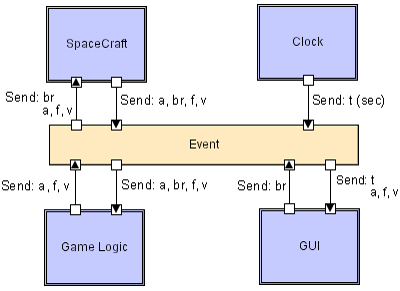
\includegraphics[width=0.55\textwidth]{eventBasedLL.png}
    \attribution{N. Medvidovic}
\end{center}

\subsection{Peer-to-peer}

Стиль <<Peer-to-peer>>, или одноранговая сеть, --- стиль, при котором система состоит из большого количества приложений, каждое из которых в принципе может само решать все задачи и является самодостаточным, но чем больше приложений работают совместно, тем шире возможности системы. Компоненты в таком стиле --- это отдельные приложения, которые имеют своё состояние, свой поток управления и всё, что нужно для работы. В качестве соединителей, как правило, выступают сетевые протоколы, а в качестве элементов данных --- сообщения по сети. 

Топологических ограничений на связи между компонентами не накладывается, даже наоборот, приветствуются избыточные связи. Кроме того, предполагается, что топология сети может динамически изменяться во время работы. компоненты могут выходить из сети или появляться новые.

Основное преимущество Peer-to-peer --- это отказоустойчивость. Можно хоть физически уничтожить часть системы, остальная часть продолжит работать, хоть и менее эффективно. Ещё такую систему легко масштабировать, просто динамически подключая к сети новые компоненты, что делает peer-to-peer идеальным для распределённых вычислений, особенно в ситуациях, когда каждый участник никому ничего не должен и работает в сети только когда у него есть возможность.

Самый, пожалуй, известный пример peer-to-peer-системы --- это BitTorrent, где каждый узел может работать как файловый сервер, но чем больше узлов, тем больше информации можно хранить и тем быстрее её можно скачивать. Есть и менее известные применения, например, сенсорные сети или стаи беспилотников, применяющиеся в военной или природоохранной сферах. Если один из беспилотников вышел из строя, стая переконфигурируется и продолжает выполнение задания.

Lunar Lander в виде сети из зондов, приземляющихся на Луне, мог бы быть устроен так:

\begin{center}
    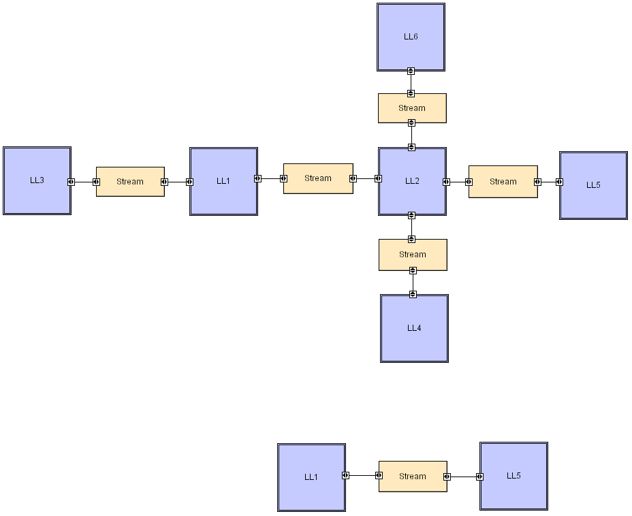
\includegraphics[width=0.9\textwidth]{peerToPeerLL.png}
    \attribution{N. Medvidovic}
\end{center}

Подробнее про Peer-to-peer мы поговорим, когда будем рассматривать архитектуру распределённых приложений.

\subsection{Гетерогенные стили}

Гетерогенные стили --- это условное название для более специфичных арххитектурных стилей, являющихся уточнением и соединением нескольких стилей, упоминавшихся ранее. Примеры таких стилей --- REST (Representational State Transfer), про который в этом курсе будет позже, Components and Connectors, стиль <<распределённые объекты>> и его конкретная реализация CORBA. Вообще, CORBA --- это конкретный стандарт (к тому же, безнадёжно устаревший на данный момент), но его авторы настолько серьёзно подошли к архитектурным аспектам, что он заслуживает тут упоминания.

\subsubsection{Components and Connectors (C2)}

Components and Connectors --- это вариант стиля с неявным вызовом, событийный стиль с шиной  плюс уровневый стиль. Есть компоненты ---- независимые, потенциально параллельные производители или потребители сообщений. Есть соединители ---  маршрутизаторы сообщений, которые могут фильтровать, преобразовывать и рассылать сообщения двух видов: нотификации и запросы. Нотификации анонсируют изменения в состоянии, содержат данные про суть изменений. Запросы --- запрашивают выполнение действия.

Стиль хорош тем, что накладывает жёсткие топологические ограничения на запросы и нотификации: нотификации шлются только <<вниз>>, а запросы только <<вверх>>. Это и привносит уровневую структуру.

Lunar Lander в таком стиле мог бы быть спроектирован вот так:

\begin{center}
    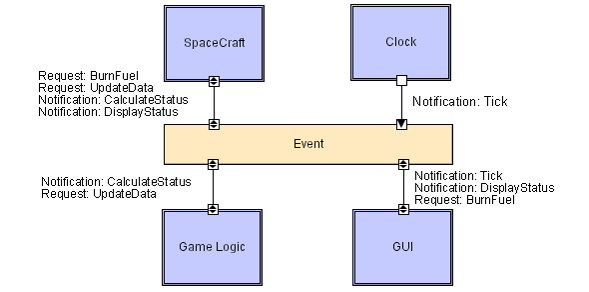
\includegraphics[width=0.7\textwidth]{c2LL.png}
    \attribution{N. Medvidovic}
\end{center}

\subsubsection{CORBA (на самом деле, <<распределённые объекты>>)}

CORBA (Common Object Request Broker Architecture) --- это конкретный стандарт, разработанный консорциумом OMG (тем самым, который стоит за UML) аж в начале 90-х. Задачей стандарта было определить протоколы и типовую архитектуру систем, состоящих из объектов, работающих на разных хостах под управлением разных операционных систем и написанных на разных языках программирования. CORBA была реализована в Java и стала очень популярна в информационных системах 90-х, но потом потеснена веб-сервисами на SOAP, а затем и REST-сервисами.

Компонентами в такой архитектуре выступают обычные объекты, каждый из которых запущен, возможно, в своём отдельном процессе и снабжён инфраструктурой для сериализации/десериализации и обработки сетевых запросов (это делает обычно какое-то заранее написанное middleware). В качестве соединителей выступают сетевые протоколы удалённого вызова, связывающие объекты с Object Request Broker (который выступает чем-то вроде шины между объектами, так что CORBA можно считать смесью событийного стиля с шиной и чистого объектно-ориентированного стиля). Никаких других топологических ограничений не накладываается.

При этом есть дополнительные инфраструктурные ограничения, связанные с сетевой природой архитектурного стиля (и делающие идею <<а давайте возьмём обычное приложение и сделаем каждый объект веб-сервисом>> экстремально плохой, кстати). Во-первых, все данные, передаваемые при вызовах (параметры, возвращаемые значения и исключения) должны быть сериализуемы. Во-вторых, каждый объект должен уметь обрабатывать ошибки сети и спокойно относиться к временной недоступности сотоварищей. То есть каждый удалённый вызов должен сам обрабатывать сетевые ошибки.

Преимущества такого стиля, на самом деле типичные для более-менее любой распределённой архитектуры --- это независимость от конкретной технологии реализации. Вы можете каждый объект писать на том языке, который вам больше нравится, лишь бы сервис поддерживал стандарт. Более того, каждый объект может быть физически расположен где угодно, хоть на другом конце света, и работать на самом разном железе. Что даёт масштабируемость, гибкость и т.д., но и добавляет разных проблем типа необходимости аккуратного деплоя.

Lunar Lander в таком стиле мог бы выглядет как-то так:

\begin{center}
    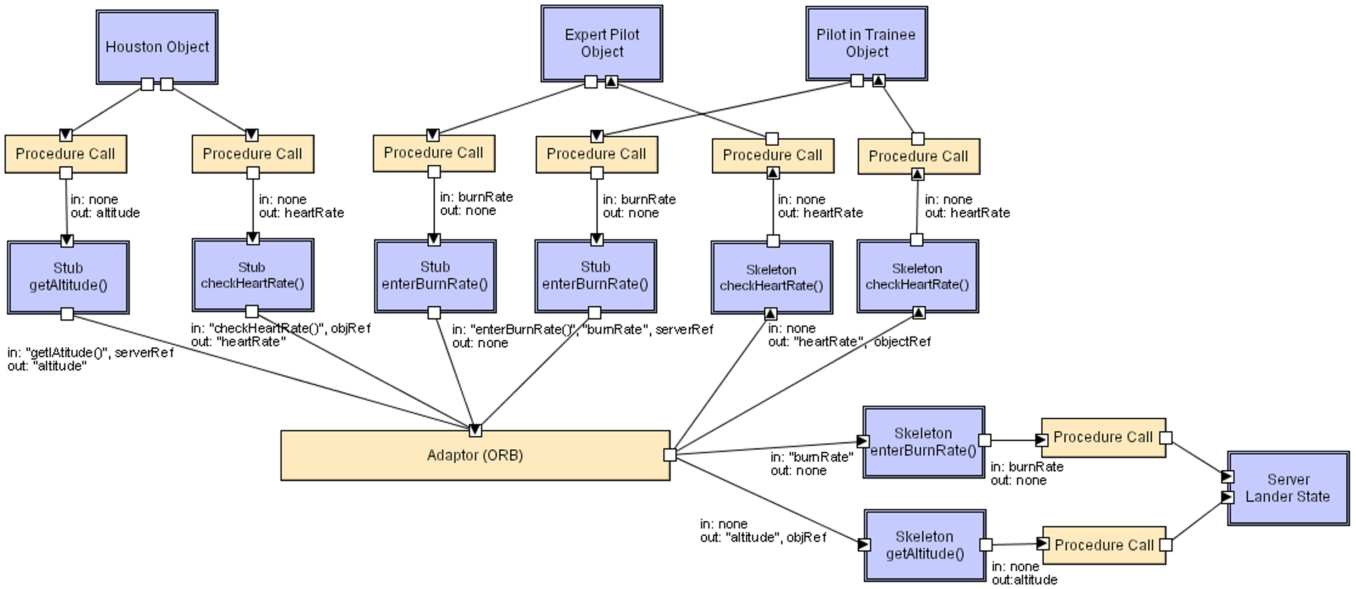
\includegraphics[width=0.9\textwidth]{corbaLL.png}
    \attribution{N. Medvidovic}
\end{center}

Про распределённые объекты мы тоже подробнее поговорим ближе к концу курса, когда речь пойдёт про архитектуру распределённых приложений.

\end{document}